\chapter[Analyse fonctionnelle]{Analyse fonctionnelle}

\textit{Le présent chapitre a pour objectif de présenter la structuration de l'application et ses principales fonctionnalités.}

\section{Contraintes principales du projet}

Les principales contraintes de développement de l’interface sont liées à la modélisation du problème. Deux choix sont possibles : une modélisation multi-classe, et une modélisation multi-label. Dans le premier cas, les objets classés sont répartis dans plusieurs classes, tout en sachant qu’un objet ne peut appartenir à deux classes différentes. Dans le cas de la modélisation multi-label, un objet peut appartenir à plusieurs classes, chacune ne proposant qu’un choix binaire (appartenance/non-appartenance). C’est une généralisation de la modélisation multi-classe.\newline

\begin{figure}[!h]
	\begin{center}
		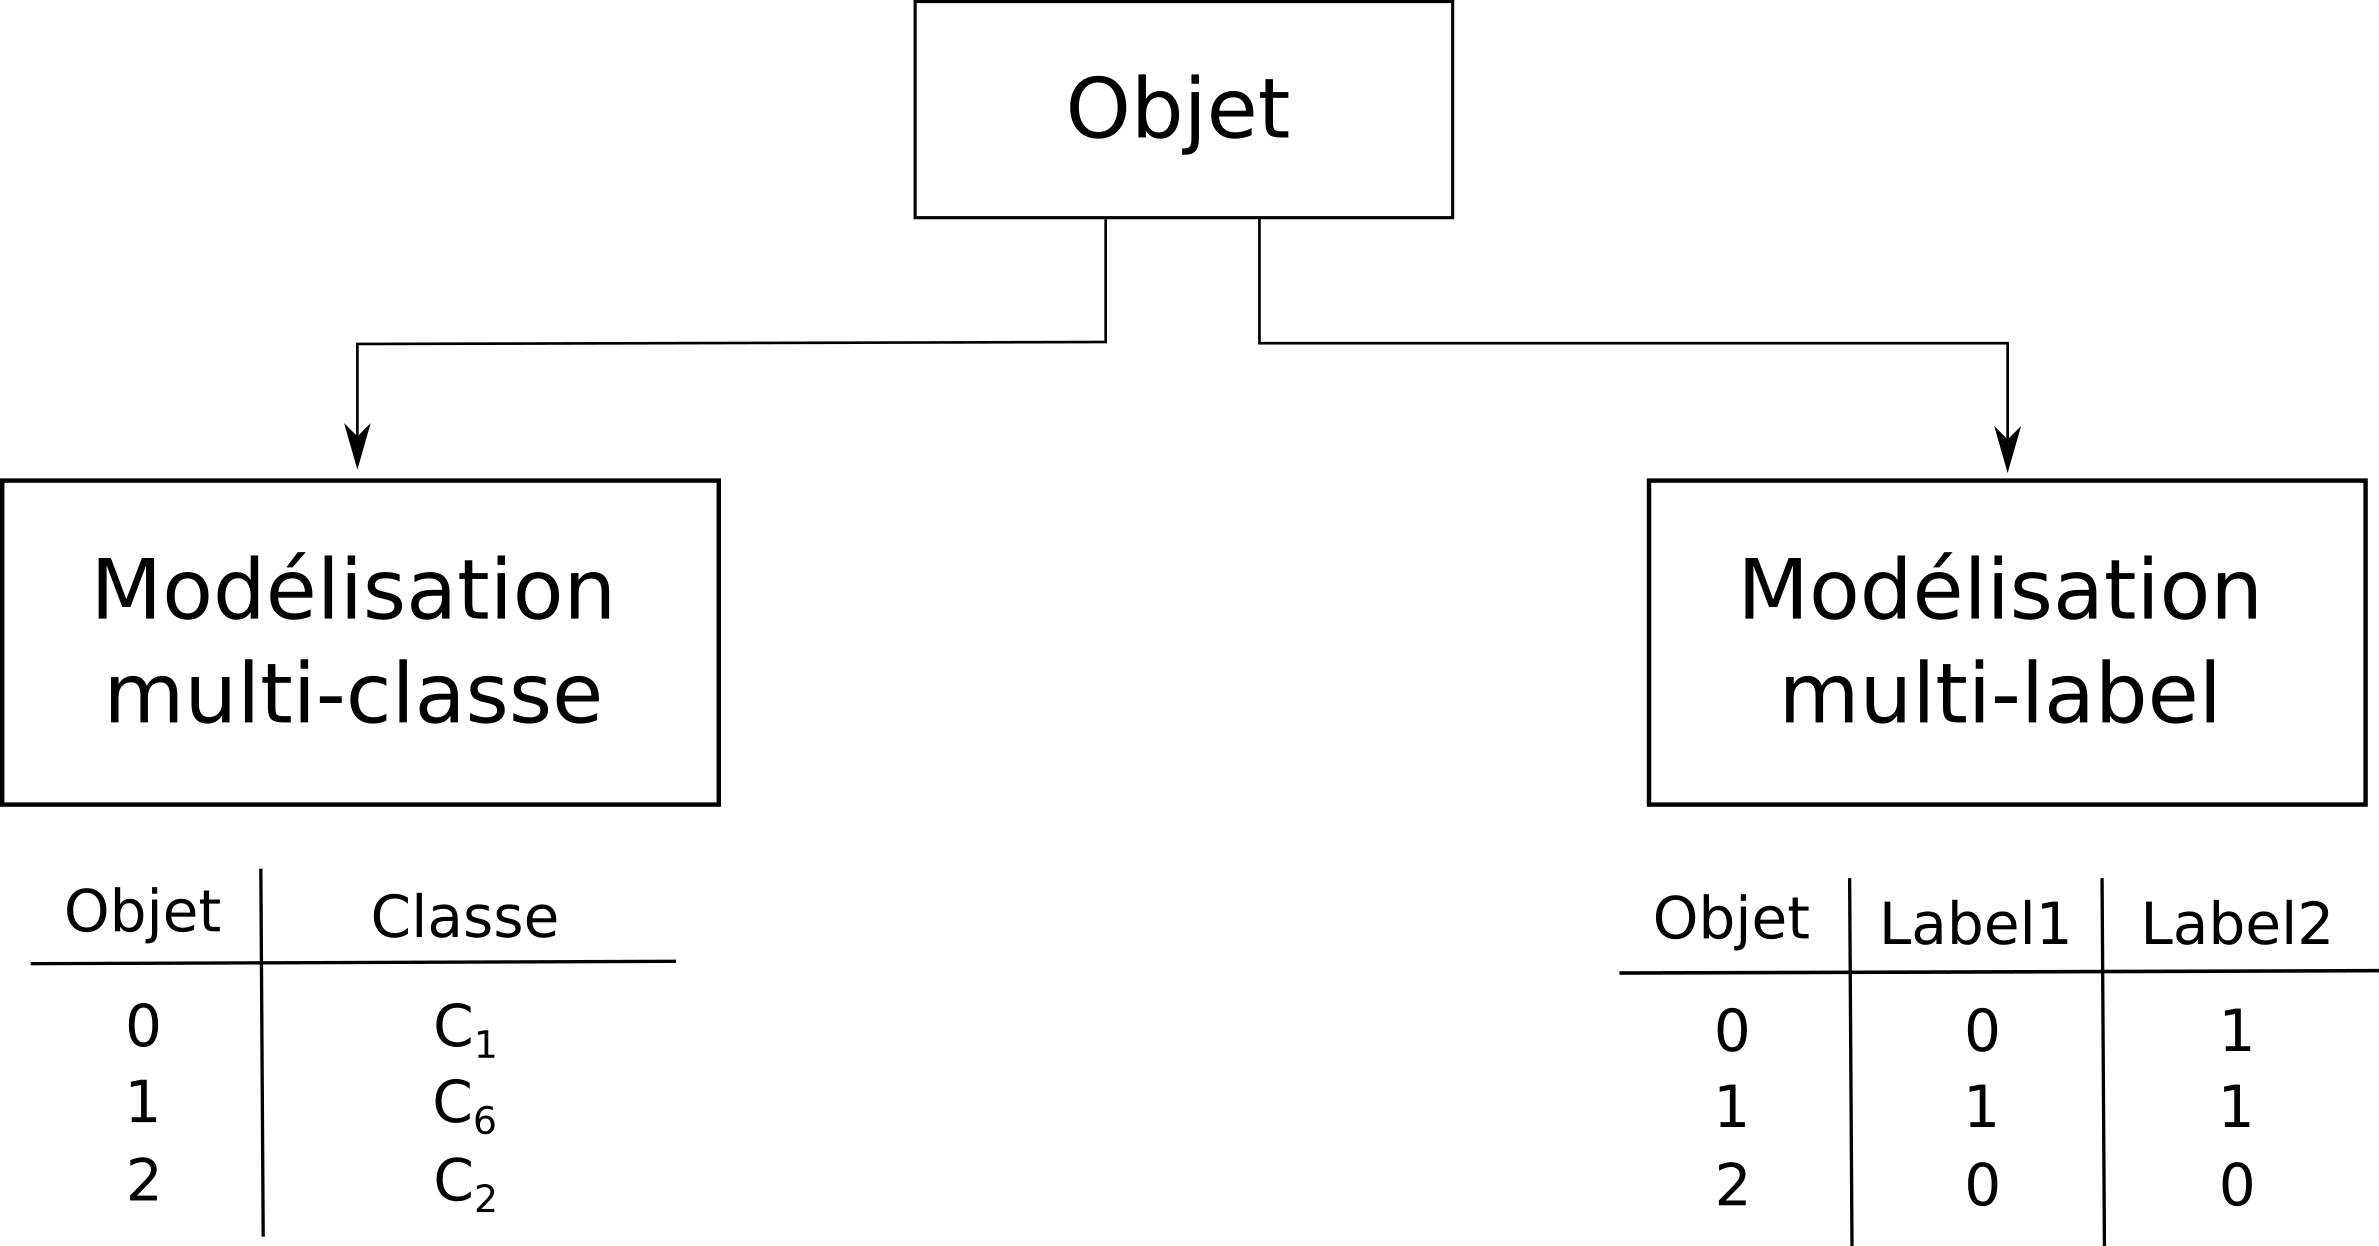
\includegraphics[scale=0.5]{modelisation.png}  \\
		\caption[Modélisation du problème]{Modélisation du problème}
		\label{fig:modelisation}
	\end{center}
\end{figure}

Le choix de la modélisation du problème a un impact sur le formalisme des données en entrée et en sortie du programme. Le choix de l’interface à montrer sera aussi déterminé par la modélisation. Ainsi, dans le cas multi-classe, un objet classifié ne sera lié qu’à une seule classe, ce qui impliquera de n’afficher que la classe concernée dans l’interface.\newline

Pour la première implémentation de l’interface, le modèle multi-classe a été privilégié pour faciliter la manipulation des données. Cependant, l’objectif est d’évoluer vers une modélisation multi-label du problème : l’interface programmée doit donc être flexible pour prendre en compte les différents formalismes. \newline

\section{Organisation des données}

\subsection{Données en entrée}

Dans une première modélisation du problème, on considère 4 jeux de données en entrée du programme :
\begin{itemize}[label=$\rightarrow$]
	\item \textbf{Un fichier « classes.CSV »}, regroupant l’ensemble des classes d’erreur, suivies d’une brève description du type d’erreur.
	\item \textbf{Un fichier « resultats.CSV »}, regroupant les résultats de la phase de classification. On retrouve donc le numéro de l’entité, la classe qui lui est associée et une probabilité d’appartenance à cette classe.
	\item \textbf{Un dossier « emprise »}, regroupant les emprises des entités au format shapefile. L’identifiant de l’entité se retrouve dans le nom du fichier d'emprise (ex : « 2516.SHP » pour l’entité 2516).
	\item \textbf{Une orthoimage au format TIFF} de la zone analysée, spatialement superposable aux fichiers d’emprise au format .SHP.\newline
\end{itemize}


L’ensemble de ces données doit être fourni par l’utilisateur avant l’exécution du programme. Pour cela, une fenêtre de chargement des fichiers doit être implémentée. \newline

\textbf{Aperçu de la fenêtre de chargement}

\subsection{Données en sortie}

En sortie de l'interface, un seul fichier est retourné :
\begin{itemize}[label=$\rightarrow$]
	\item \textbf{Un fichier « modifyresults.CSV »}, regroupant les résultats de l'interaction avec l'utilisateur, sous une forme identique au fichier « results.CSV ». Deux méthodes sont envisageables : une première hypothèse consiste à sortir un tableau avec l'ensemble des entités testées (qu'elles soient modifiées ou non), et une seconde à ne restituer que les entités qui ont été modifiées.\newline
\end{itemize}

\noindent\textit{Question : même si l'utilisateur confirme la classification, la probabilité est quand même modifiée et passe à 1 car on est sur de la classe ?! Il faudrait donc considérer toutes les entités traitées dans le fichier de sortie }

\subsection{Structuration des données}

\noindent\textbf{Lecture et écriture des fichiers .CSV}\\

Les données au format .CSV (Comma-Separated Values) concernent les fichiers « classes» et « resultats ». Ce format permet d’enregistrer des données lignes par lignes en séparant les valeurs par une virgule. \newline

Dans le programme, les fichiers seront traduits de manières différentes :

\begin{itemize}[label=$\rightarrow$]
	\item Pour le fichier « classes », les données seront enregistrées dans une variable de type dictionnaire. A la différence des listes, cet objet n’a pas de structure ordonnée, et il est possible d’accéder à ses entités grâce à des clés. Dans notre cas, les clés contiendront l’identifiant des listes. On choisit de ne pas créer de classe car ces données sont très peu susceptibles d’évoluer.
	\item Pour le fichier « resultats », les données seront enregistrées comme une liste d’objets « Resultat ». Cette nouvelle classe « Resultat » permettra de créer des entités logiques, composée d’un identifiant, d’une classe, d’une probabiltié, et liées à une emprise. Ces objets seront également utilisés pour écrire le fichier des résultats finaux (« resultatsModifies.CSV »)
\end{itemize}

\noindent\textbf{Lecture du fichier d’emprise .SHP}\\

Le format shapefile est un format de fichier pour les systèmes d'informations géographiques (SIG). Il contient toutes les informations liées à la géométrie de l’entité. (\textit{gestion du repère d’affichage par la fenêtre graphique de QT ??})\\

La lecture de ce fichier permet de compléter une liste d’objets « Emprise ». Cette classe permettra de créer un objet composé d’un identifiant, d’une géométrie, et de ses bornes d’affichage.\\

\noindent\textbf{Lecture de l’orthophotographie au format .TIFF}\\

Une seule orthophoto est fournie en entrée du calcul. Il n’est donc pas nécessaire de créer une classe spécifique pour cet objet unique.\\

\noindent\textbf{Diagramme de classe}\\

Le projet peut être décomposé en 5 classes principales :
\begin{itemize}[label=$\rightarrow$]
	\item La classe Resultat
	\item La classe Emprise
	\item Les 3 classes correspondant aux 3 interfaces (fenêtre principale, fenêtre de chargement des fichiers, fenêtre de reclassement des entités)\\
\end{itemize}

\begin{figure}[!h]
	\begin{center}
		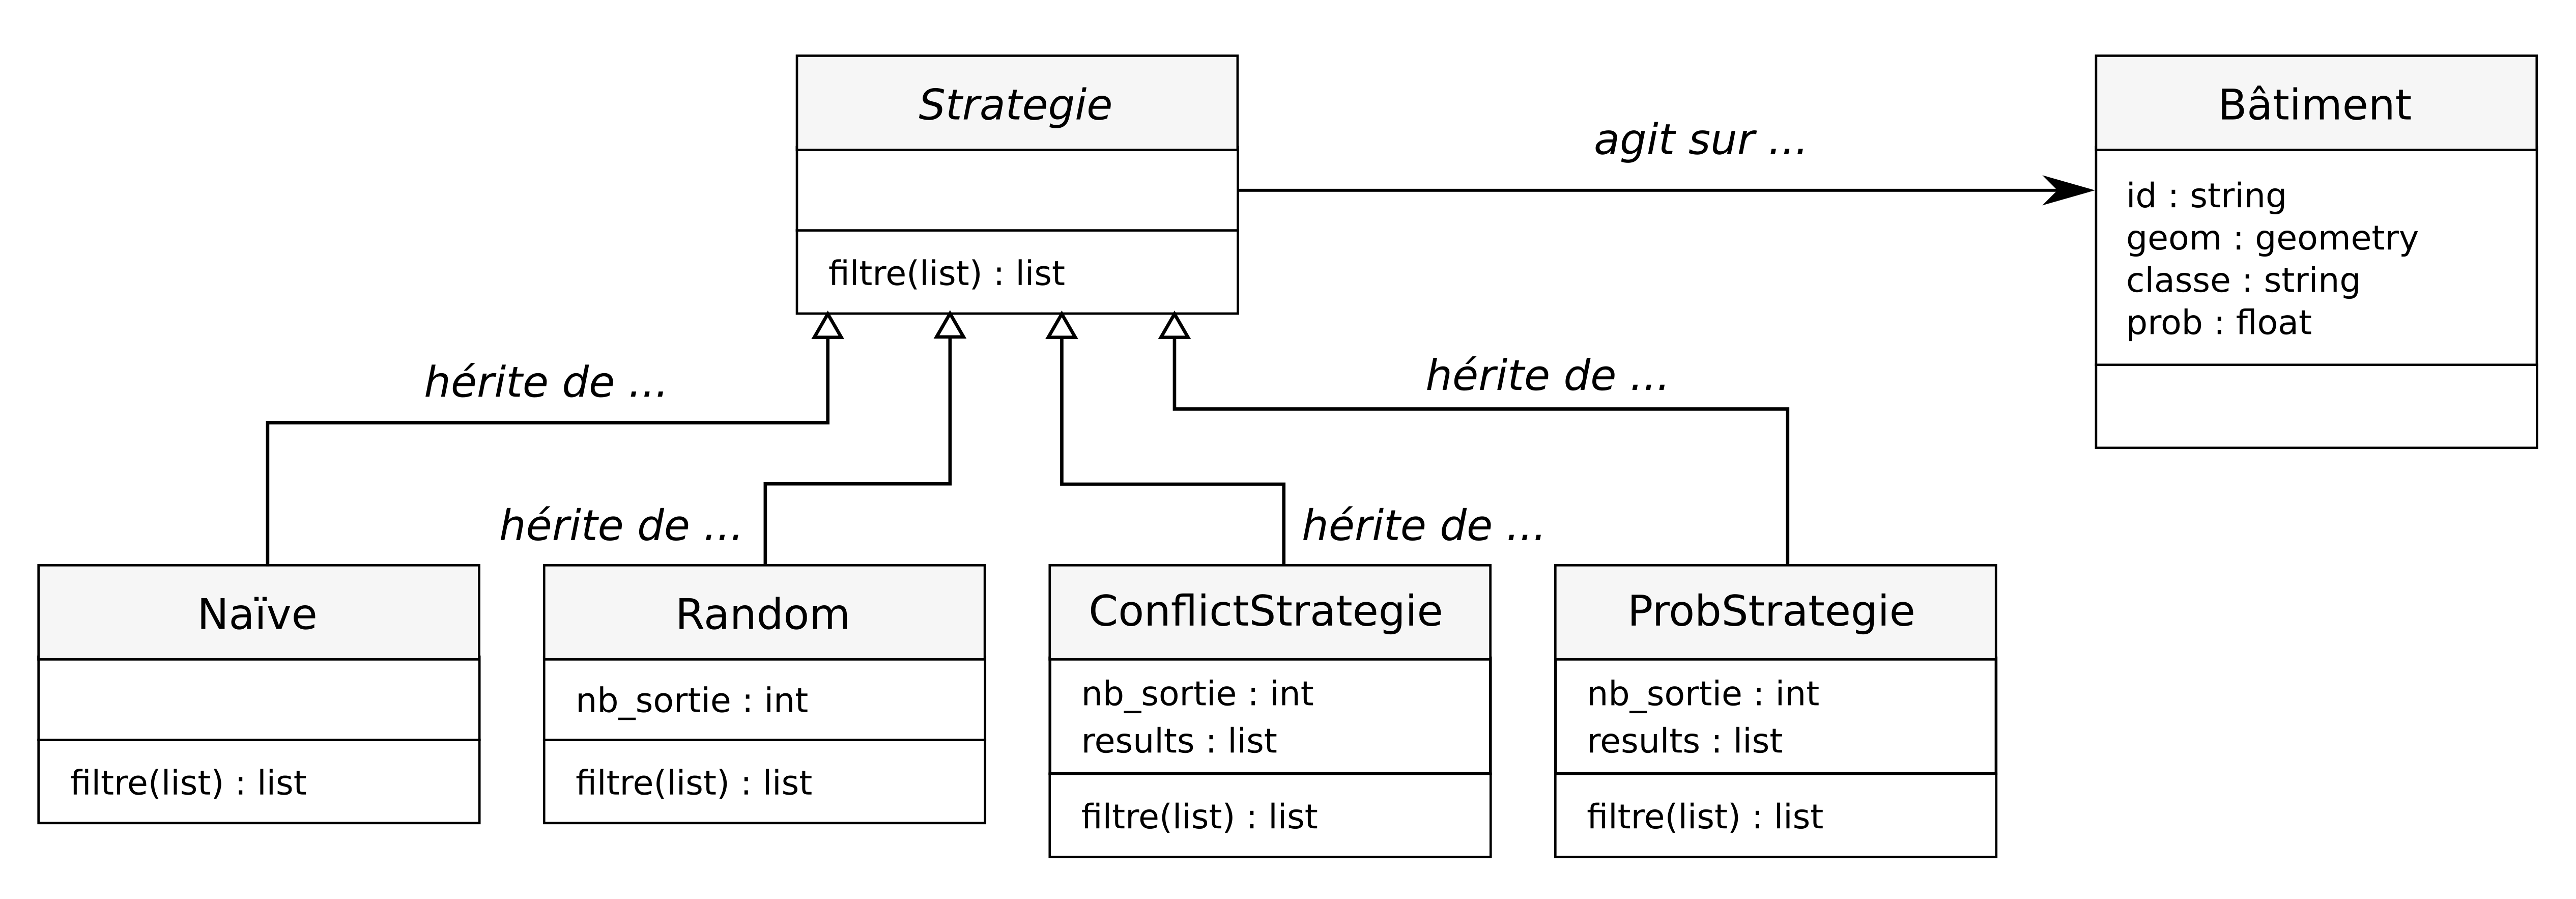
\includegraphics[scale=0.5]{diagramme_classes.png}  \\
		\caption[Diagramme de classe]{Diagramme de classe}
		\label{fig:classe}
	\end{center}
\end{figure}



\newpage

\section{Analyse fonctionnelle}

\subsection{Principales fonctionnalités du programme}

L'interface doit permettre de visualiser et contrôler les résultats d'une classification.

\begin{figure}[h]
	\begin{center}
		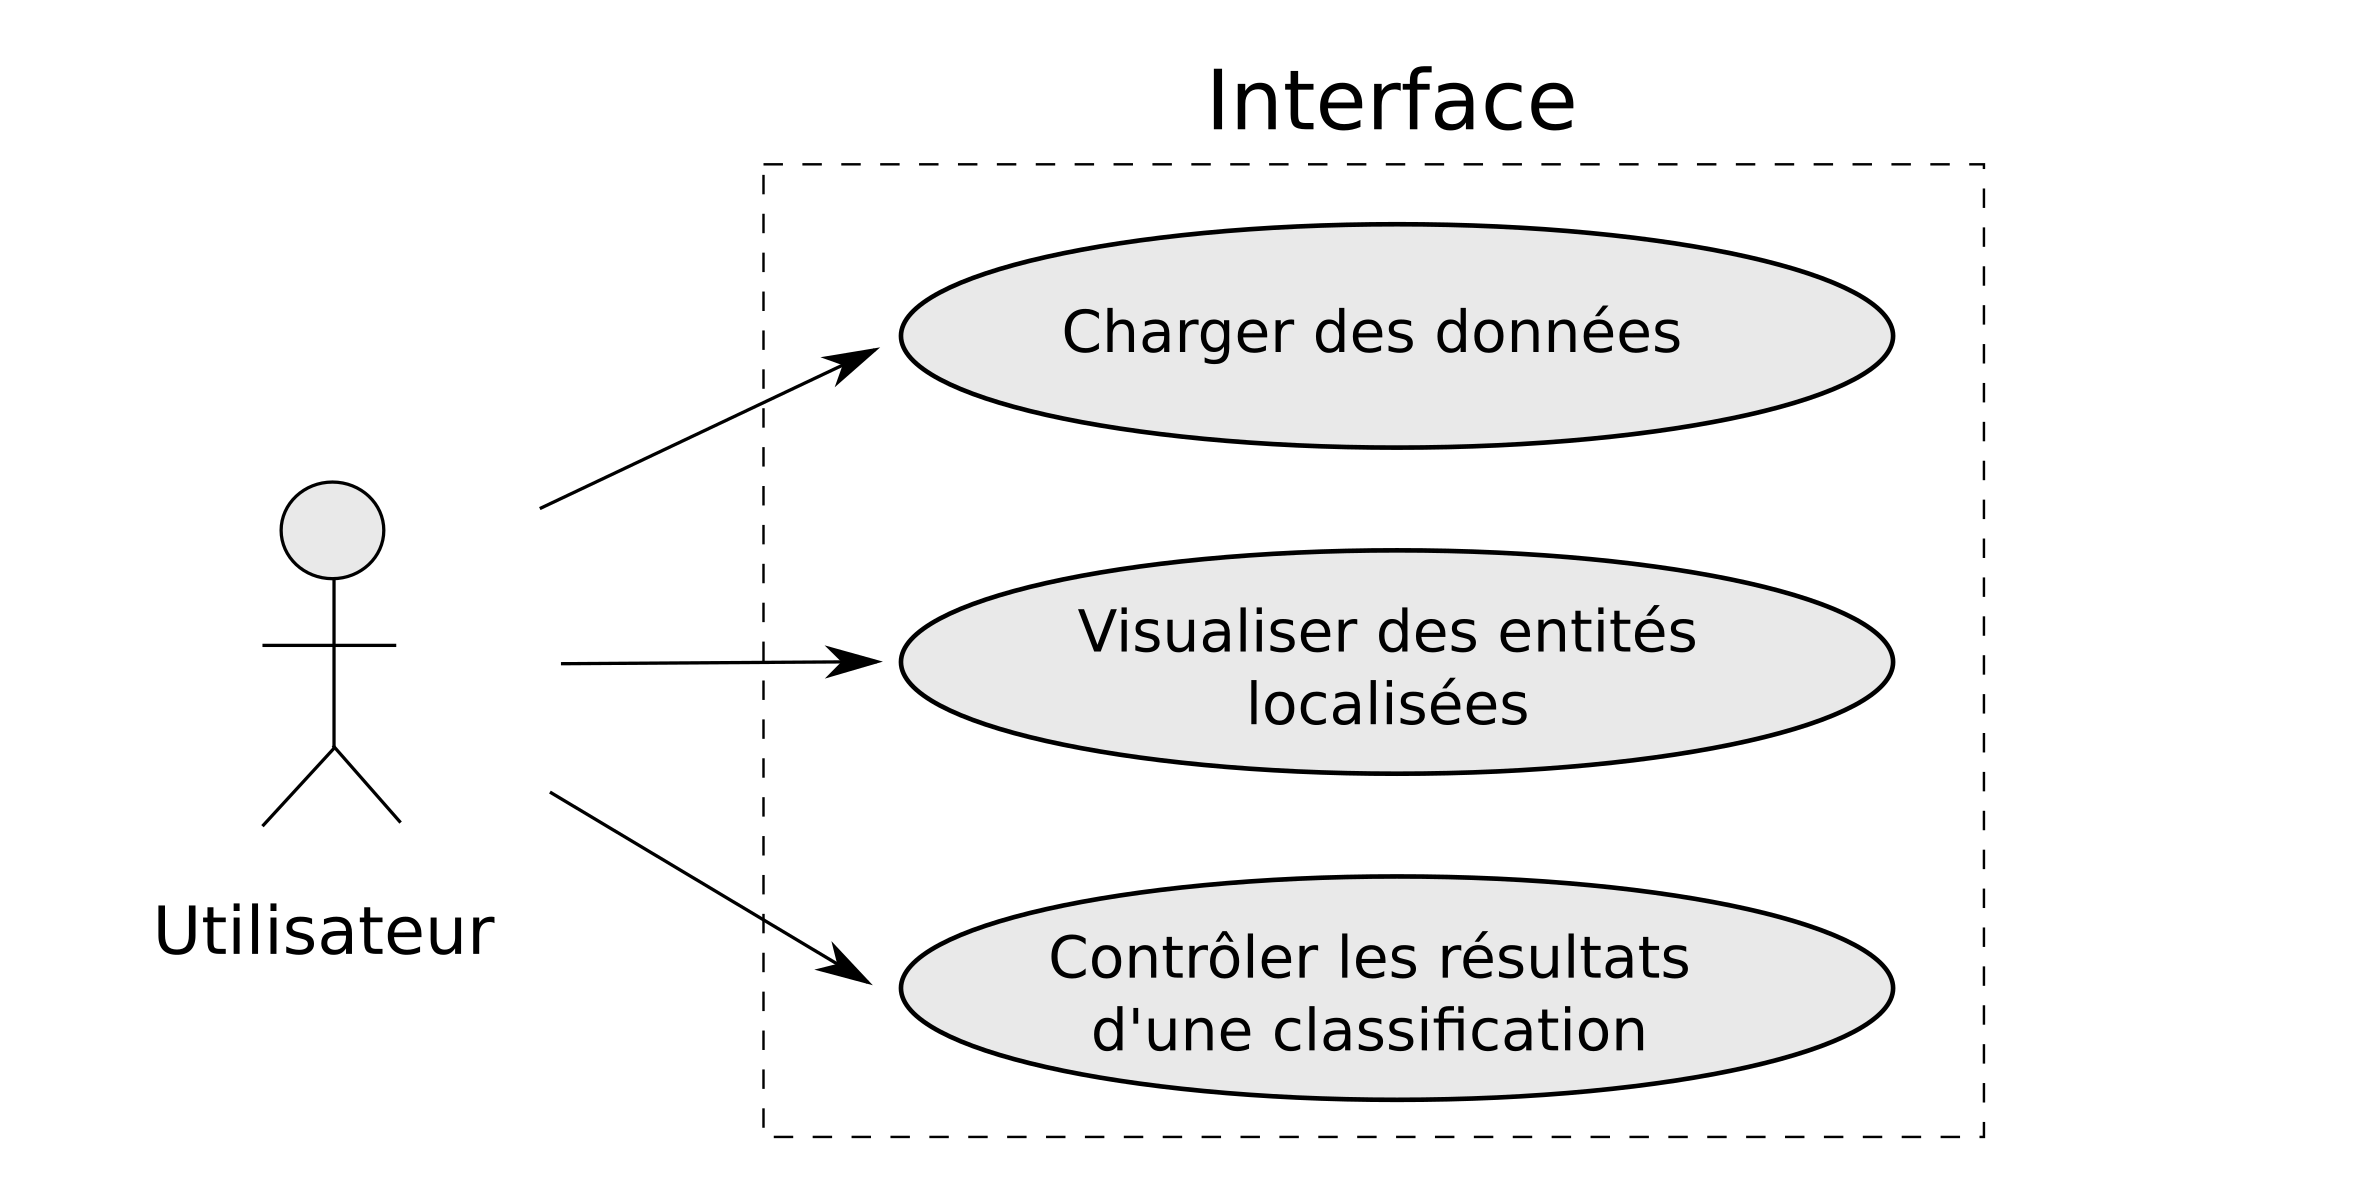
\includegraphics[scale=0.6]{diagramme_cas_utilisation.png}  \\
		\caption[Cas d'utilisation]{Cas d'utilisation}
		\label{fig:utilisation}
	\end{center}
\end{figure}


\subsection{Organisation des fonctions}

\noindent\textbf{Diagramme fonctionnel}\\

\begin{figure}[!h]
	\begin{center}
		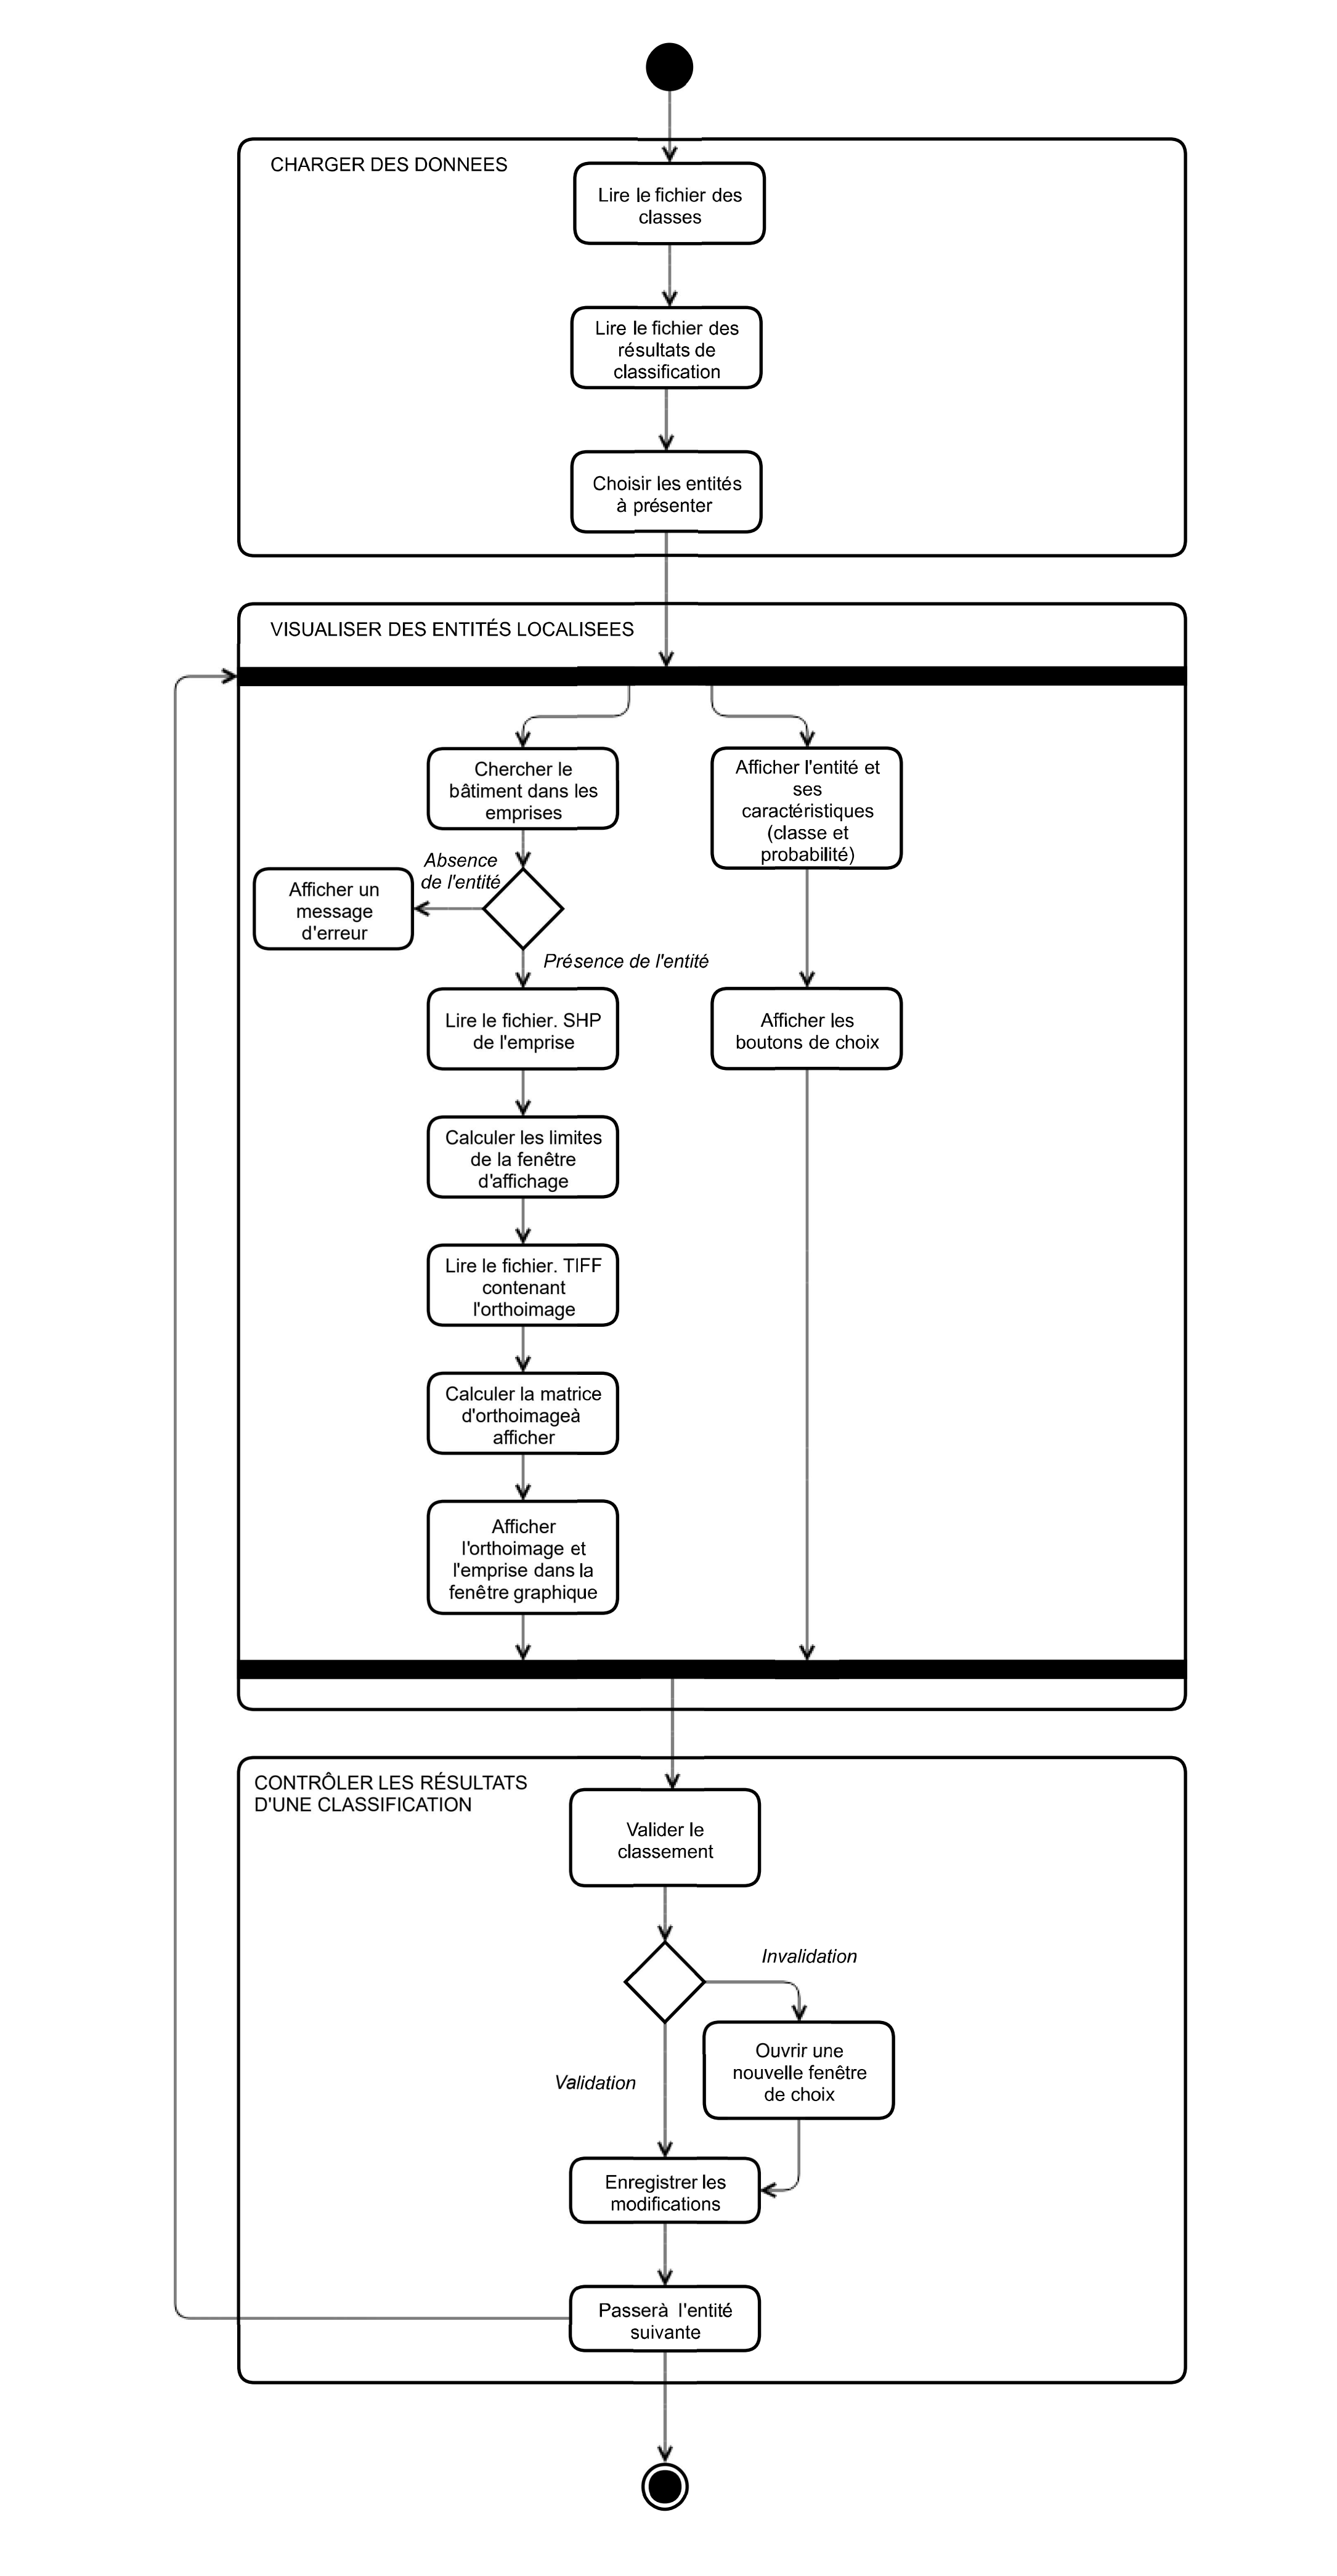
\includegraphics[scale=0.8]{Analyse_fonctionnelle.png}  \\
		\caption[Diagramme fonctionnel]{Diagramme fonctionnel}
		\label{fig:fonction}
	\end{center}
\end{figure}


\noindent\textbf{Fonction de sélection des entités}\\

Cette fonction doit permettre à l’utilisateur de choisir la stratégie d’affichage des entités résultant de la classification. En effet, l’objectif n’est pas que l’utilisateur contrôle l’ensemble des données, mais seulement celles qui influent le plus sur la classification.\newline

Trois stratégies principales d’affichages peuvent être envisagées :
\begin{enumerate}
	\item L’affichage de toutes les entités
	\item L’affichage des entités dont la probabilité d’appartenance est la plus faible
	\item L’affichage des entités ayant des conflits de classification (cas des entités ayant plusieurs erreurs, mauvaise qualification des erreurs, …)\newline
\end{enumerate}

Dans les deux derniers cas, des entités aléatoires devront également être affichées. En effet, si l’on souhaite améliorer le processus global de classification, l’utilisateur doit agir sur toutes les classes.\\ 

Deux types de traitement sont envisageables : 
\begin{enumerate}
	\item Un traitement offline, qui sélectionne les entités à afficher indépendamment de la requalification par l’utilisateur
	\item Un traitement online, qui va sélectionner un échantillon de donnée qui va être remis à jour selon les résultats du reclassement\newline
\end{enumerate}

Dans un premier temps, on se limitera à l’affichage de toutes les entités d’un fichier de manière offline afin de se concentrer sur le fonctionnement global de l’interface.


\noindent\textbf{Manipulation des fichiers d'emprise}\\

L’ensemble des fichiers .SHP correspondant aux emprises sont stocké dans un dossier unique. Une première étape sera donc de lire ces fichiers pour associer chaque objet « Resultat » à une emprise, en utilisant l’identifiant. Dans la première implémentation, en cas d’absence de l’emprise dans le dossier, cette fonction devra afficher une fenêtre d’erreur à l’utilisateur.\newline

Une deuxième étape consistera à calculer, pour chaque emprise, les bornes d’affichage qui lui sont liées. Cela nécessite de déterminer la fenêtre d’affichage ([$x_{min}$,$y_{min}$] et [$x_{max}$,$y_{max}$]) lors de la lecture du fichier. Les marges ($m_x$,$m_y$) définies par l’utilisateur sont ensuite rajoutées aux coordonnées pour obtenir les angles repères de la fenêtre graphique ([$x_h$,$y_h$] et [$x_b$,$y_b$]).\newline

\begin{figure}[!h]
	\begin{center}
		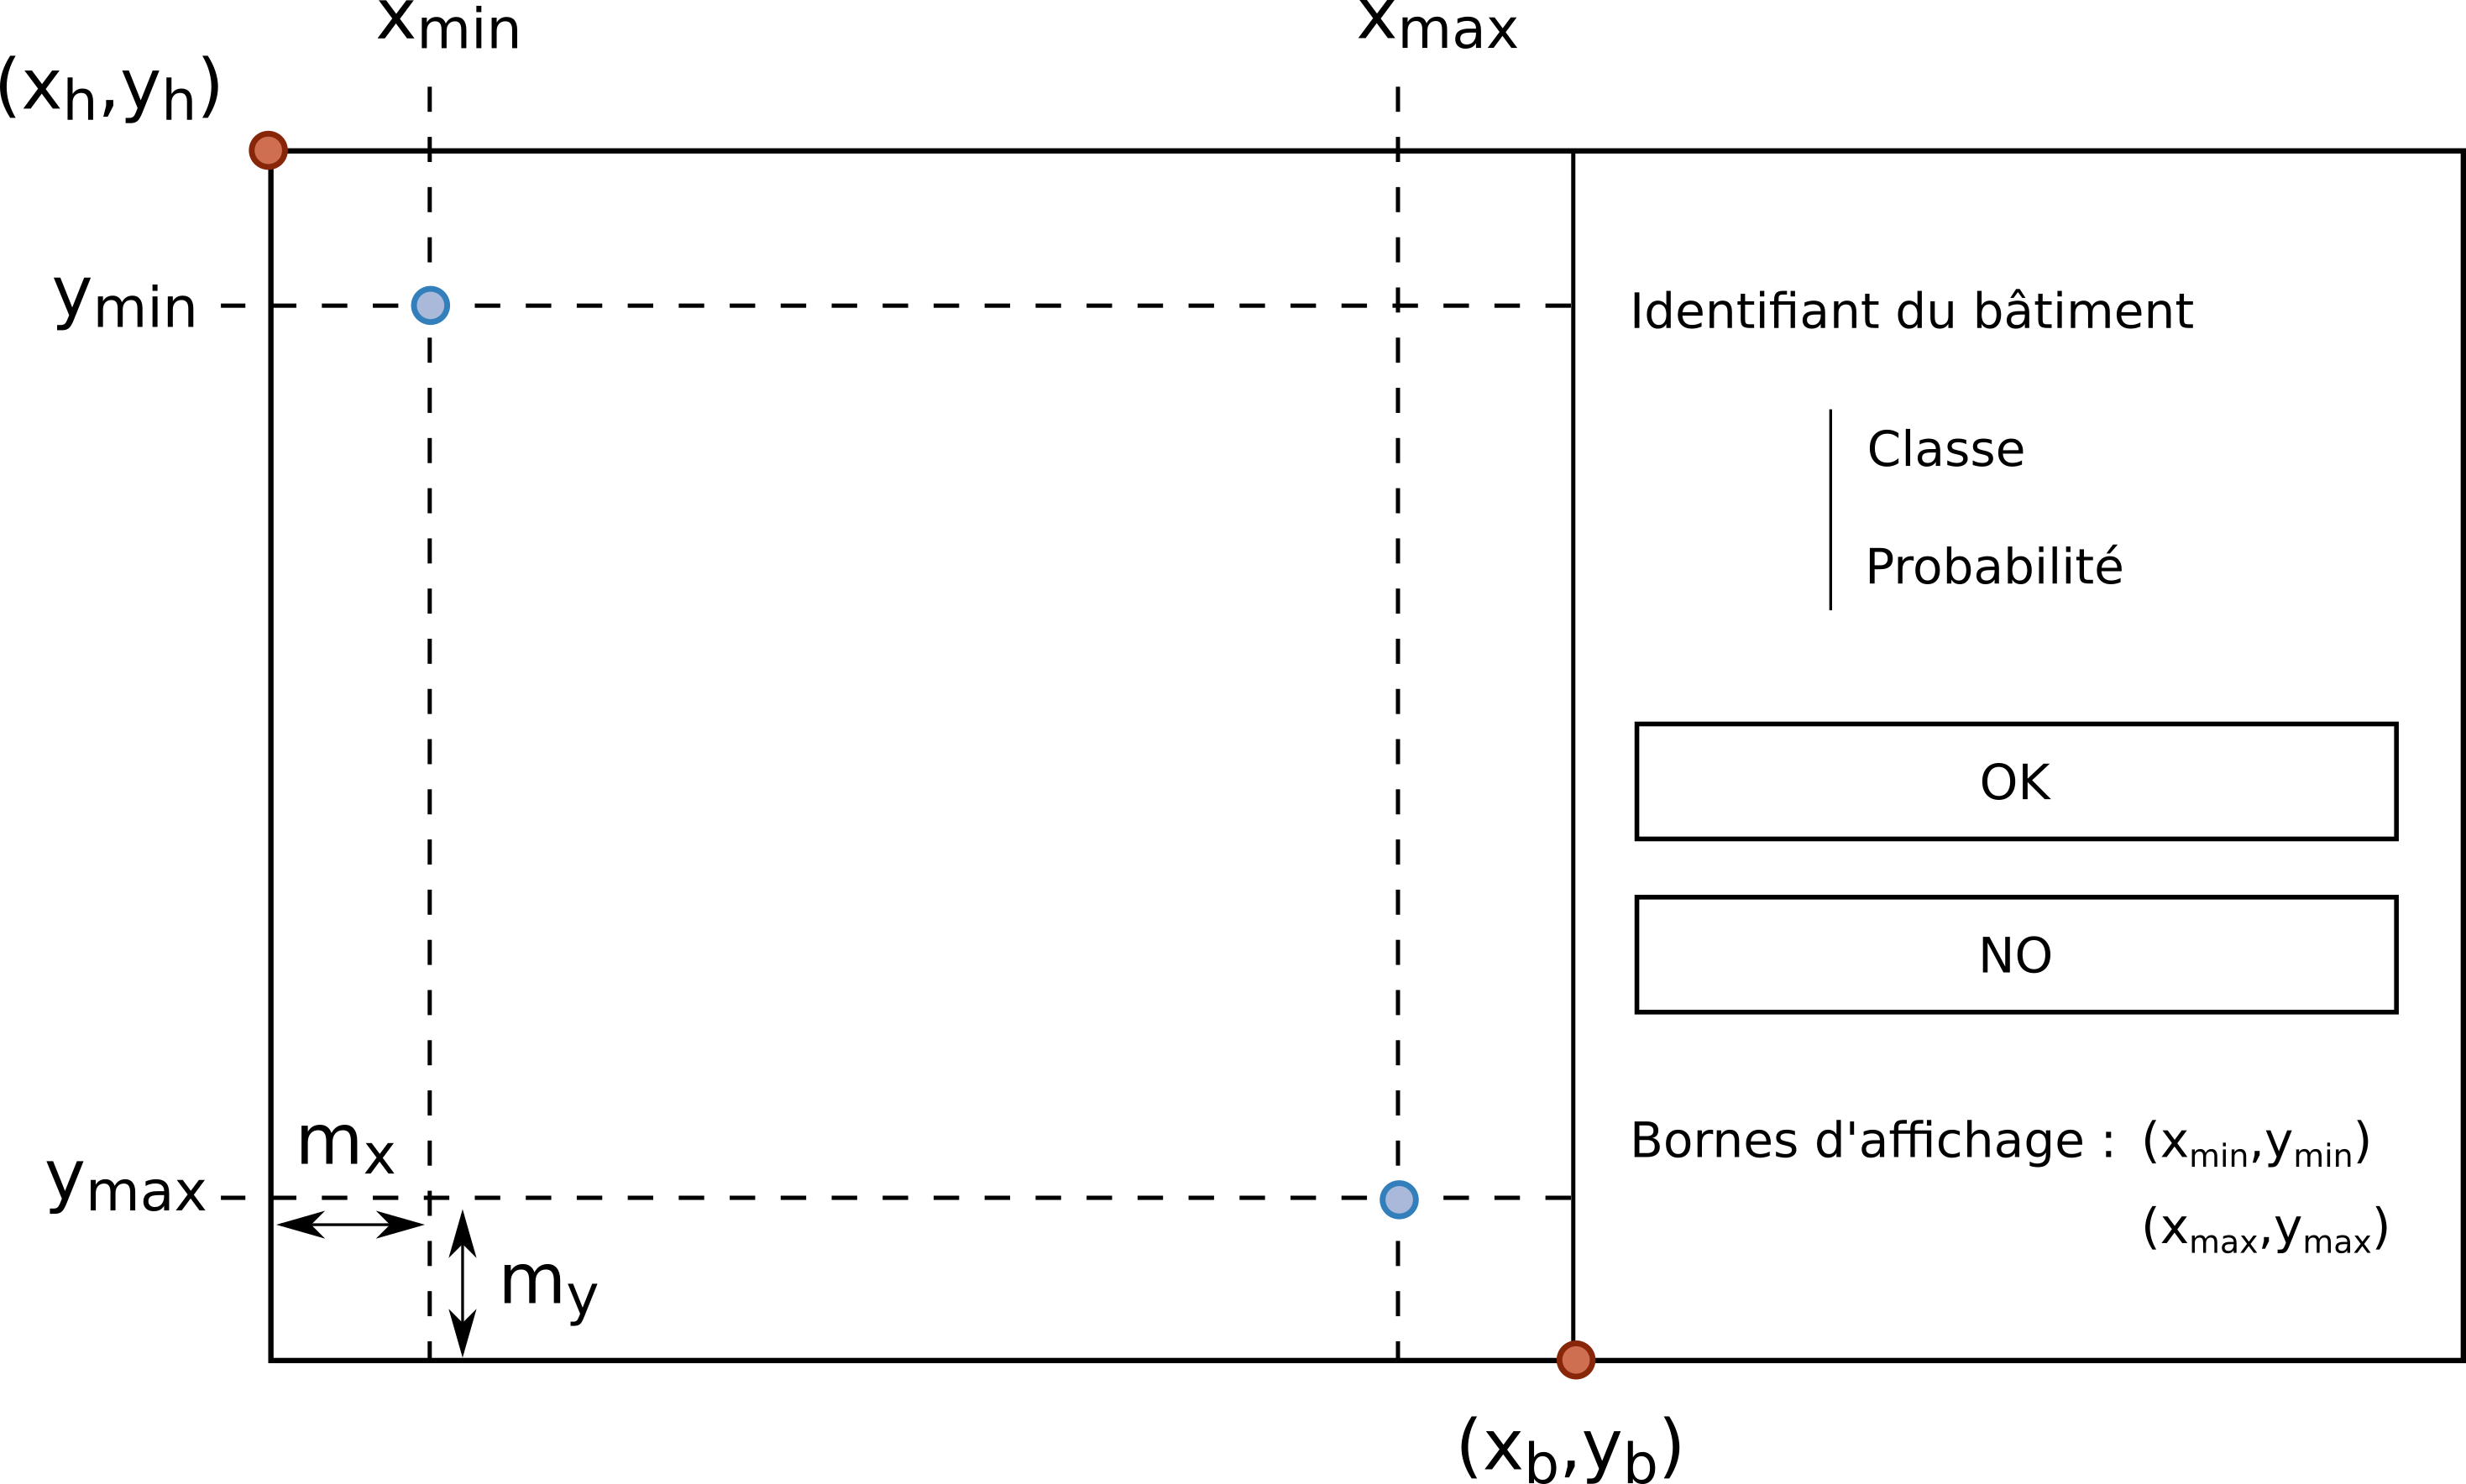
\includegraphics[scale=0.4]{interface_schema.png}  \\
		\caption[Schéma d'organisation de l'interface]{Schéma d'organisation de l'interface}
		\label{fig:interfaceschema}
	\end{center}
\end{figure}

\noindent\textbf{Analyse de l'orthoimage}\\

La lecture du fichier .TIFF de l’orthoimage doit nous permettre de trouver le point d’origine de l’ortho, ainsi que la taille d’un pixel. Les emprises étant spatialement superposables à l’orthoimage, on utilise les valeurs des bornes d’affichage des emprises pour calculer la matrice d’orthoimage à afficher. Dans la fenêtre graphique, on lui superpose l’emprise du bâtiment.\newline

\noindent\textbf{Phase d'interaction avec l'utilisateur}\\

L’affichage des informations relatives à l’entité dans l’interface permet à l’utilisateur de contrôler les résultats de la classification :
\begin{itemize}[label=$\rightarrow$]
	\item Si l’utilisateur valide le résultat, le résultat est enregistré et la fenêtre affiche l’entité suivante.
	\item Si l’utilisateur invalide le résultat, une nouvelle fenêtre s’ouvre et propose les autres choix possibles. L’utilisateur ne peut sélectionner qu’une seule proposition, puis valide. Le résultat est enregistré et la fenêtre affiche l’entité suivante.
\end{itemize}

\subsection{Conception de l'interface}

Pour faciliter l’écriture et la compréhension du code de l’interface, on utilisera la méthode Modèle/Vue/Contrôleur :

\begin{itemize}[label=$\rightarrow$]
	\item Le fichier « Modèle » contiendra les données à afficher en entrée et les résultats attendus en sortie;
	\item Le fichier « Vue » contiendra le code de l’interface graphique;
	\item Le fichier « Contrôleur » contiendra les définitions informatiques des actions effectuées par l’utilisateur dans l’interface (ex : actions à exécuter lors de la validation de la classification, …). Il modifiera les données contenues dans « Modèle », ce qui va entrainer un changement dans la « Vue ».
\end{itemize}

\begin{figure}[!h]
	\begin{center}
		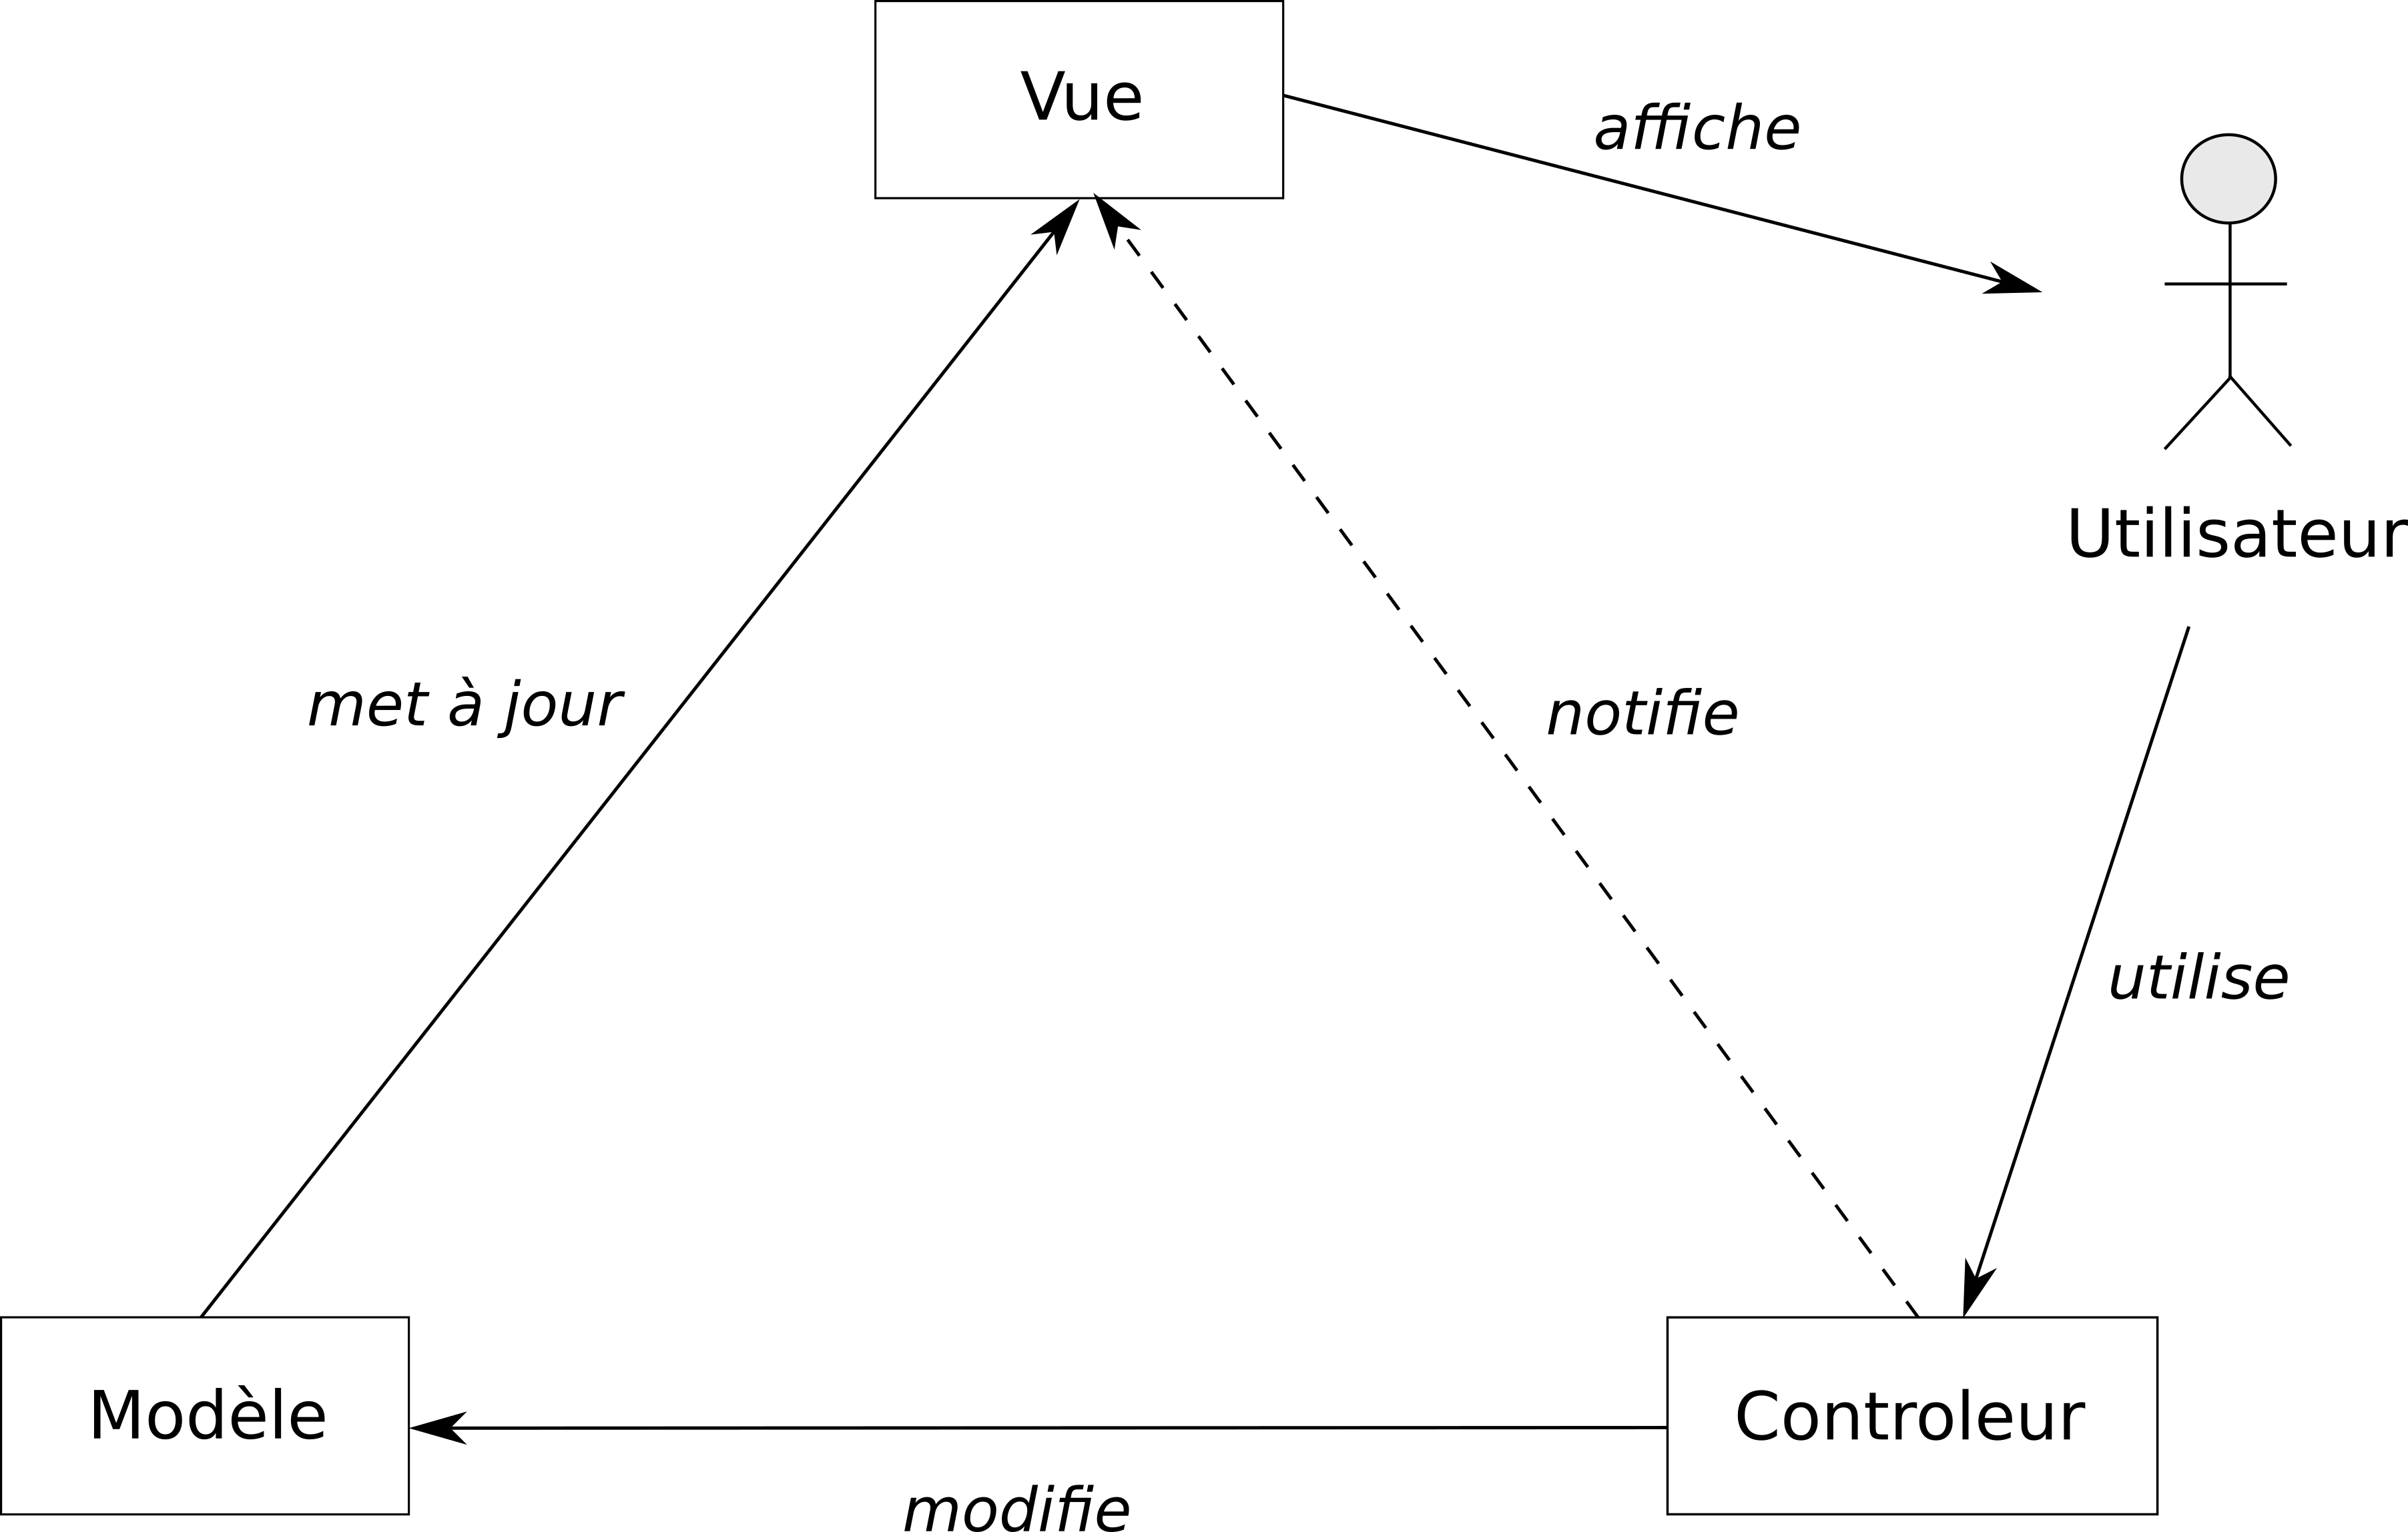
\includegraphics[scale=0.25]{MVC.png}  \\
		\caption[Agencement Modèle/Vue/Contrôleur]{Agencement Modèle/Vue/Contrôleur}
		\label{fig:MVC}
	\end{center}
\end{figure}

\subsection{Maquette du projet}




